% !TeX root = ../main.tex
% Add the above to each chapter to make compiling the PDF easier in some editors.


\chapter{Conclusions}\label{chapter:conclusion}

In this work, we obtained an imperative implementation
of B-Trees that is capable to handle queries whether a key is contained
and queries to insert new keys.
Concrete code has been obtained in the languages Scala and SML,
where the code generator may simply be extended to support other languages.
We have proven it functionally correct with the help of an abstract
specification that is refined by the imperative code.
The abstract specification fully implements
a Set interface in Isabelle, also including deletion of elements.

\section{Working in Isabelle}

An overview on the resulting theory modules
and their relationship to external modules and one another
can be seen in \Cref{fig:thm-relationships}.
The given graphic roughly resembles the actual file structure.
It can be seen that in order to develop this project
not many general lemmas and definitions had to be added to the library.
The library of proofs considered here
is the one provided by the Isabelle/HOL framework together with the \textit{Archive of Formal Proofs}.
The latter is a refereed collection of proofs that contains, among others,
the separation logic framework.

\begin{figure}
    \centering
    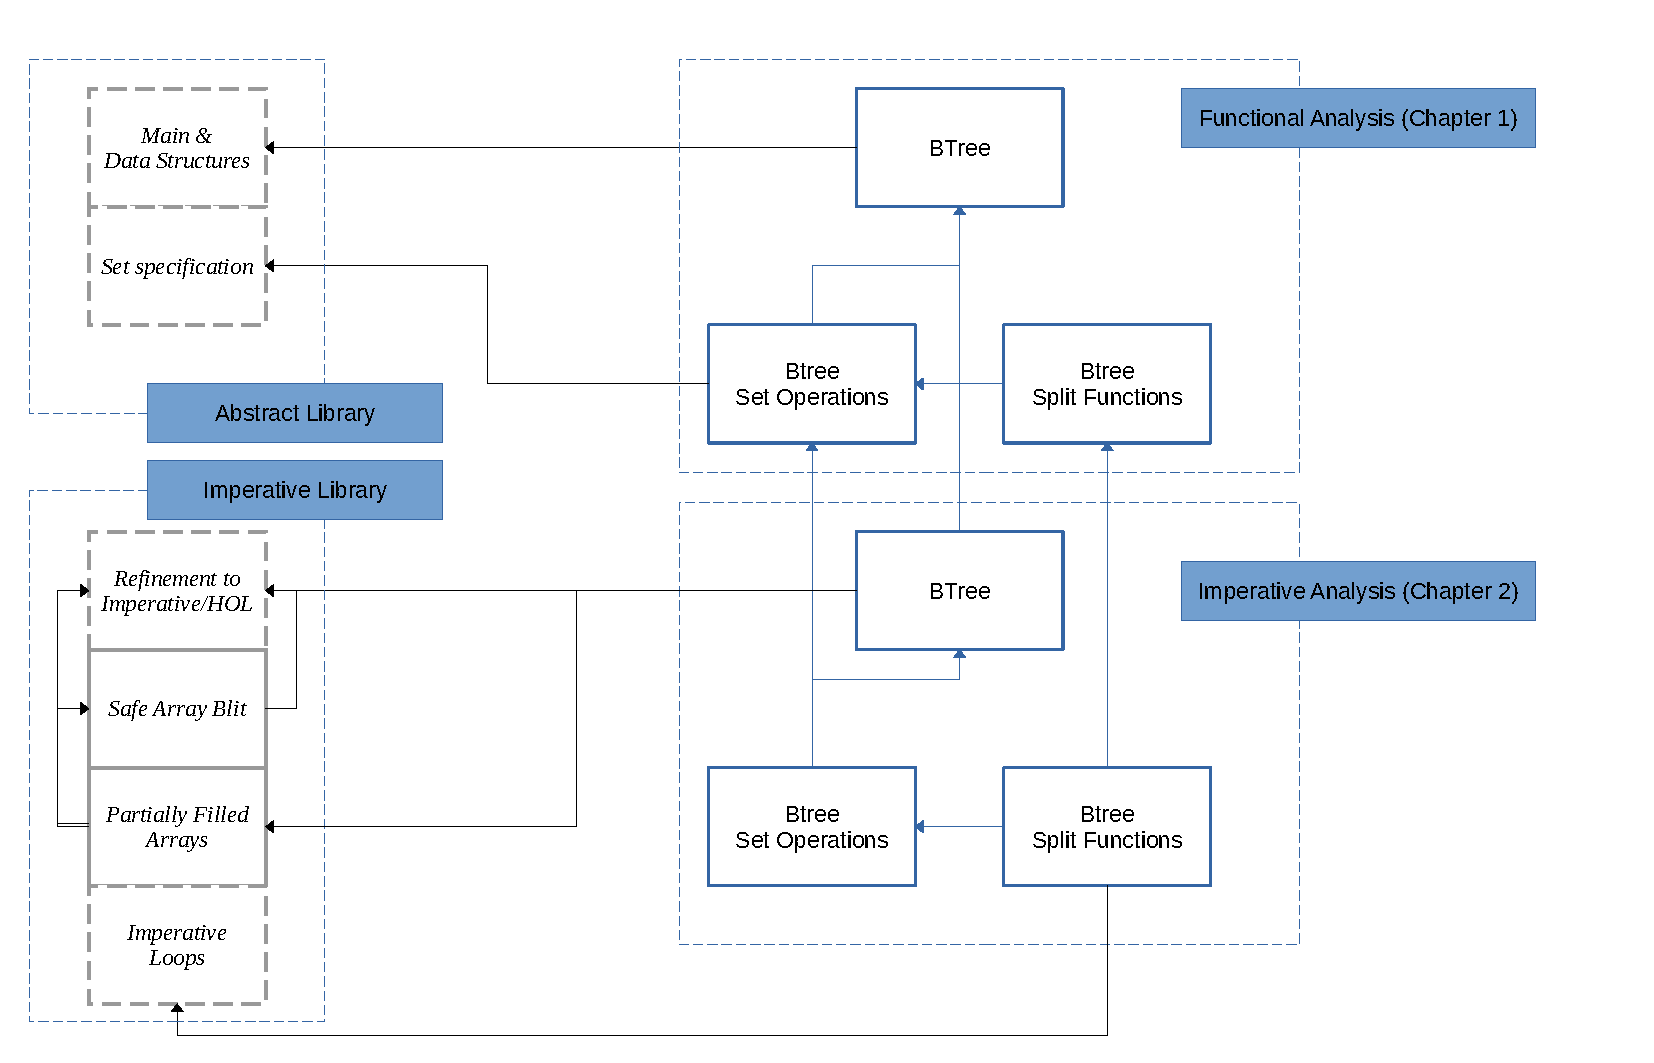
\includegraphics[width=1.1\linewidth]{figures/theories-relationship.pdf}
    \caption[An overview on the theories comprised by this work
    and their approximate relationship.]{
    An overview on the theories comprised by this work
    and their approximate relationship.
    An arc points to a theory or package
    that contains required lemmas or definitions.
    Theories created or significantly extended in the course of this work are outlined with a continuous line.}
    \label{fig:thm-relationships}
\end{figure}

One main source of frustration is finding the correct
functions and lemmas to apply for proofs.
While in natural proofs a certain kind of function and corresponding equalities can be
expected to be known by the reader.
However for machine checked proofs, as the only meaningful way,
all used lemmas need to be provided.
Now usually the Isabelle/HOL provides tools like sledgehammer
or \textbf{find\_theorems} in order to find useful lemmas for the concrete situation.
However each have their own drawbacks.

If the goal is only to simplify a given expression but not to
directly solve the result, sledgehammer is useless
as it only returns the applied lemmas for a successfully finalized proof.
This would have been especially useful for the apply style proofs of the
imperative implementation, that was mainly comprised of simplification steps.
Maybe the tools can be extended to return what lemmas lead to promising
simplifications of the the goal term to provide additional input to the user.

Secondly \textbf{find\_theorems} is useless if the current state
is simplified too much to not perfectly match the required lemma anymore.
As a concrete example, the $inorder$ of B-Trees was first defined
with "foldr map \textit{$\dots$ ts []}".
The proof system could not provide any useful lemmas on expressions of this form.
However there exists the standard function $concat$ that
simplifies to the above and has useful lemmas for catenation
and splitting.
It was only discovered close to the finalization of the thesis
when more standard terms for employed functions were searched for.
Since the available lemmas were key to a practical
implementation of the inorder set interface,
this meant a wasted workload of almost 2000 lines of additional proof.
The lesson learnt is to always look for alternative or equivalent
formulations of properties as well as lemmas,
to see what kind of existing lemmas may be employed.

Another point of discomfort is in the separation logic framework.
Especially when inserting elements in lists,
original assumptions on the whole list have to be split
into assumptions on parts of the list or lists obtained by concatenation.
The aggressive simplification of the automatic
separation logic prover (\textbf{sep\_auto})
does often go to far in these proofs.
This either results in unreadable (and unprovable)
subgoals resulting from a chain of commands.
Sometimes it also yields states for which a rule
may not be applied anymore.
For example when we apply $node_i$ on some list,
this list has usually been changed to append or insert a single element.
This means that $blist\_assn$ holds for the whole list,
however since the automation tools knows that the list
is comprised on sublists it automatically simplifies related expressions.
In order to match the resulting precondition with the $node_i$ heap rule
defined on full lists, an intermediate rule has to be derived
that has as precondition the simplified state.


% TODO note that node_i requires temporary allocation of an array that contains all elements.
% it would be more efficient to derive a specialized version that takes two arrays
% and redistributes between them evenly

% TODO this might be conclusion
In the abstract analysis part of this work,
the proofs have been written to use only
minimal requirements on the input.
For example in \Cref{lem:splitmax-inorder}, rather than
requiring balancedness and $\order k$ for $k > 0$ on the full tree,
it is only required that the node has at least two children,
the last two have equal height
and that the last tree has the same, recursive property.
Using a more specific assumption was beneficial during the proof,
as the less restrictive requirements turn up in the
induction hypothesis again and are easier to satisfy than general assumptions.
However this also called for more lemmas that show that
the weaker property is satisfied in valid B-Trees.
Nevertheless, generating the most general lemmas usually turned out to be
very useful, for example in \Cref{lem:nodei-order}, yielding the reusability of $node_i$ for
merging two nodes in deletion.
Another use case was the applicability of weaker properties
even when temporary violations
of the general invariant were observed during deletion,
such as in the \textit{del} function in \Cref{lst:del-def}.
%---------------------------------

\section{Comparison and Future Work}

% TODO note that the proof for  sortedness has been reduced from 2000 lines
% by the sorted (inorder ...) notation (and Nipkows auxiliary funs/lemmas)
% comparison standard approach and list approach
During this work, a significant difference in the effort
to proof invariants using the standard set interface
and the set interface by inorder has emerged.
The proof of the standard set interface required a number of additional functions
comprising 36 lines of code.
The bigger part however is made up by the proofs required.
Including additional auxiliary lemmas, the whole proof of sortedness
and correct set operations required a staggering over 1900 lines of proof.
The proof was complex and hardly readable due to the 
extensive use of efficient solvers.
This is opposing 5 lines for the inorder and sorted function and
483 lines of proof required for the inorder approach,
which is mostly composed of easily understandable chains of equations.


% TODO comparison with other approaches
Overall the detour via a functional specification has seemed to pay off.
We realize that the rigorous verification of B-Trees or the related B$^+$-Trees
is a hard problem.
Both Malecha and Gidon report the validity of the tree shape
and invariants such as node size or sorting
to be the most difficult properties to prove.
In our approach, a valid tree shape was directly given
by the refinement property of the algebraic B-Tree type.
The other abstract invariants could be reasoned about
in the context of the abstract specifications and as such
required a number of intermediate, but obvious
lemmas that were comparatively straightforward to obtain.
The comparison between the three proof approaches in \label{fig:proof-comparison}
shows differences both with respect to the amount of 
time invested and the amount of manually provided lines of proof.
It may seem that the detour via a rigourously implemented
functional implementation yields less complex and
simpler to prove code.
It should however be noted that the B-Tree implementation
might in itself be simpler to reason about than B$^+$-Trees.

\begin{figure}
    \centering
    \begin{tabular}{l|c|c|c}
        \                & \parencite{DBLP:conf/popl/MalechaMSW10}$^{+}$ & \parencite{DBLP:journals/sosym/ErnstSR15}$^{+d}$ & Our approach \\
        \hline
        Functional code &   360      & -                    & 324  \\
        Imperative code &   510      & 1862                  & 170  \\
        Proofs          &  5190      & 350 + 510 + 2940\footnotemark[1] & 2753 \\
        Timeframe (months) &  -     & 6+                      & 4   \\
    \end{tabular}
    \caption[Comparison of (unoptimized) Lines of Code and time investment in related mechanized B-Tree verifications.]
    {Comparison of (unoptimized) Lines of Code and time investment in related mechanized B-Tree verifications.
    The marker $^+$ denotes implementations of B$^+$-Trees
    and $^d$ denotes that the implementation additionally verifies deletion operations.
    }
    \label{fig:proof-comparison}
\end{figure}
\footnotetext[1]{
    The proof is done integrating TVLA and KIV, and hence comprises
    explicitely added rules for TVLA (the first number),
    user-invented theorems in KIV (the second number)
    and "interactions" with KIV (the second number).
    Interactions are i.e. choices of an induction variable, quantifier instantiation
    or application of correct lemmas.
    We hence interpret them as each one apply-Style command and hence
    one line of proof.
}

It should be noted that further,
in contrast to related work and common implementations,
this work implements B-Trees as concretizations of sets.
Usually B-Trees are rather in use as map data structures,
mapping the unique primary keys
of database tuples to stored data.
Future work could adjust the code and proofs given here
to show that similar operations on a similar structure satisfies
the map interface.
The main difference would then be that not the indices
are the main elements of the nodes but pairs of the 
index and the corresponding data or a similar
implementation of a singleton map.
We expect this to be not more than manual work,
but to cause no specific new issues.

It should be noted at this point that the obtained code is not yet
truly optimized with respect to minimal memory allocation and access.
For that, some further refinements are necessary.
For example, the imperative \textit{node$_i$} function
requires temporarily allocating
an array that has enough space to contain
all elements that are supposed to be merged or split.
Optimizing it would maybe give a function that takes
as an argument two arrays and redistributes elements between them,
or an array and an element that is to be inserted.
This naturally increases the required amount of additional,
specialized heap rules and makes the proofs more complex.
How to gradually improving the efficiency of the implementation
without greatly increasing the complexity of correctness
proofs is a topic for further research.


However it should be noted that a transfer of the results in
this work may be difficult for the related B$^+$-Tree,
providing another subject for future research.
B$+$-trees usually contain pointers to the next leaf
on the lowest level, a property that is potentially harder
to represent on a functional level than in imperative code.
It might be necessary at that point to introduce additional
invariants directly on the imperative level.